\documentclass[10pt,border=2pt]{standalone}
\usepackage[T1]{fontenc}
\usepackage{lmodern}
\usepackage{pgfplots}
\pgfplotsset{compat=1.18}
\definecolor{convexblue}{HTML}{0072B2}
\definecolor{concaveorange}{HTML}{D55E00}
\begin{document}
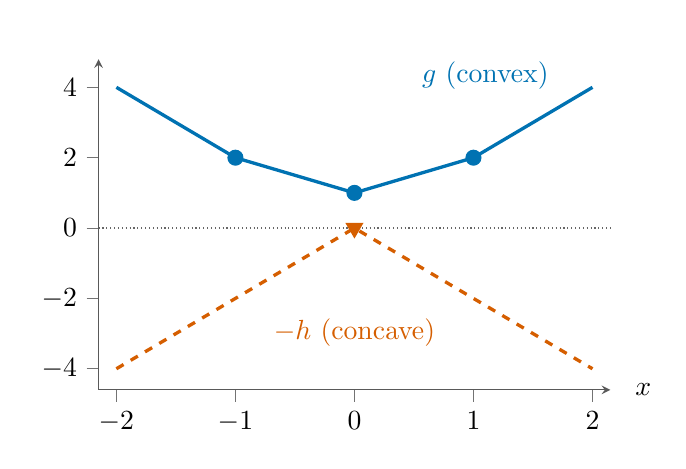
\begin{tikzpicture}
\path[use as bounding box] (-0.9,-0.65) rectangle (7.1,4.6);
\begin{axis}[
  scale only axis,width=6.5cm,height=4.2cm,
  at={(0,0)},anchor=south west,
  xmin=-2.15,xmax=2.15,xtick={-2,-1,0,1,2},
  axis lines=left,axis line style={black!65},
  tick align=outside,tick style={black!55},
  xlabel={$x$},xlabel style={at={(axis description cs:1.03,0)},anchor=west},
  label style={font=\normalsize},tick label style={font=\normalsize},
  clip=false,
  ymin=-4.6,ymax=4.8,ytick={-4,-2,0,2,4},
]
\addplot[black!60,densely dotted,thin] coordinates {(-2.15,0) (2.15,0)};
\addplot[convexblue,very thick] coordinates {(-2,4) (-1,2) (0,1) (1,2) (2,4)};
\addplot[concaveorange,very thick,dashed] coordinates {(-2,-4) (-1,-2) (0,0) (1,-2) (2,-4)};
\addplot[only marks,mark=*,mark size=2.7pt,convexblue] coordinates {(-1,2) (0,1) (1,2)};
\addplot[only marks,mark=triangle*,mark options={rotate=180},mark size=3.4pt,concaveorange]
  coordinates {(0,0)};
\node[convexblue,anchor=south] at (axis cs:1.1,3.65) {$g$ (convex)};
\node[concaveorange,anchor=north] at (axis cs:0,-2.3) {$-h$ (concave)};

\end{axis}
\end{tikzpicture}
\end{document}
